\section{Gestion des terrains}

\textbf{Si vous êtes un membre du staff, et que vous avez la permission de gérer les terrains}, vous pouvez alors accéder à la page de gestion des terrains, depuis l'onglet \enquote{Staff} tout à droite du menu de navigation.

\begin{figure}[H]
\centering
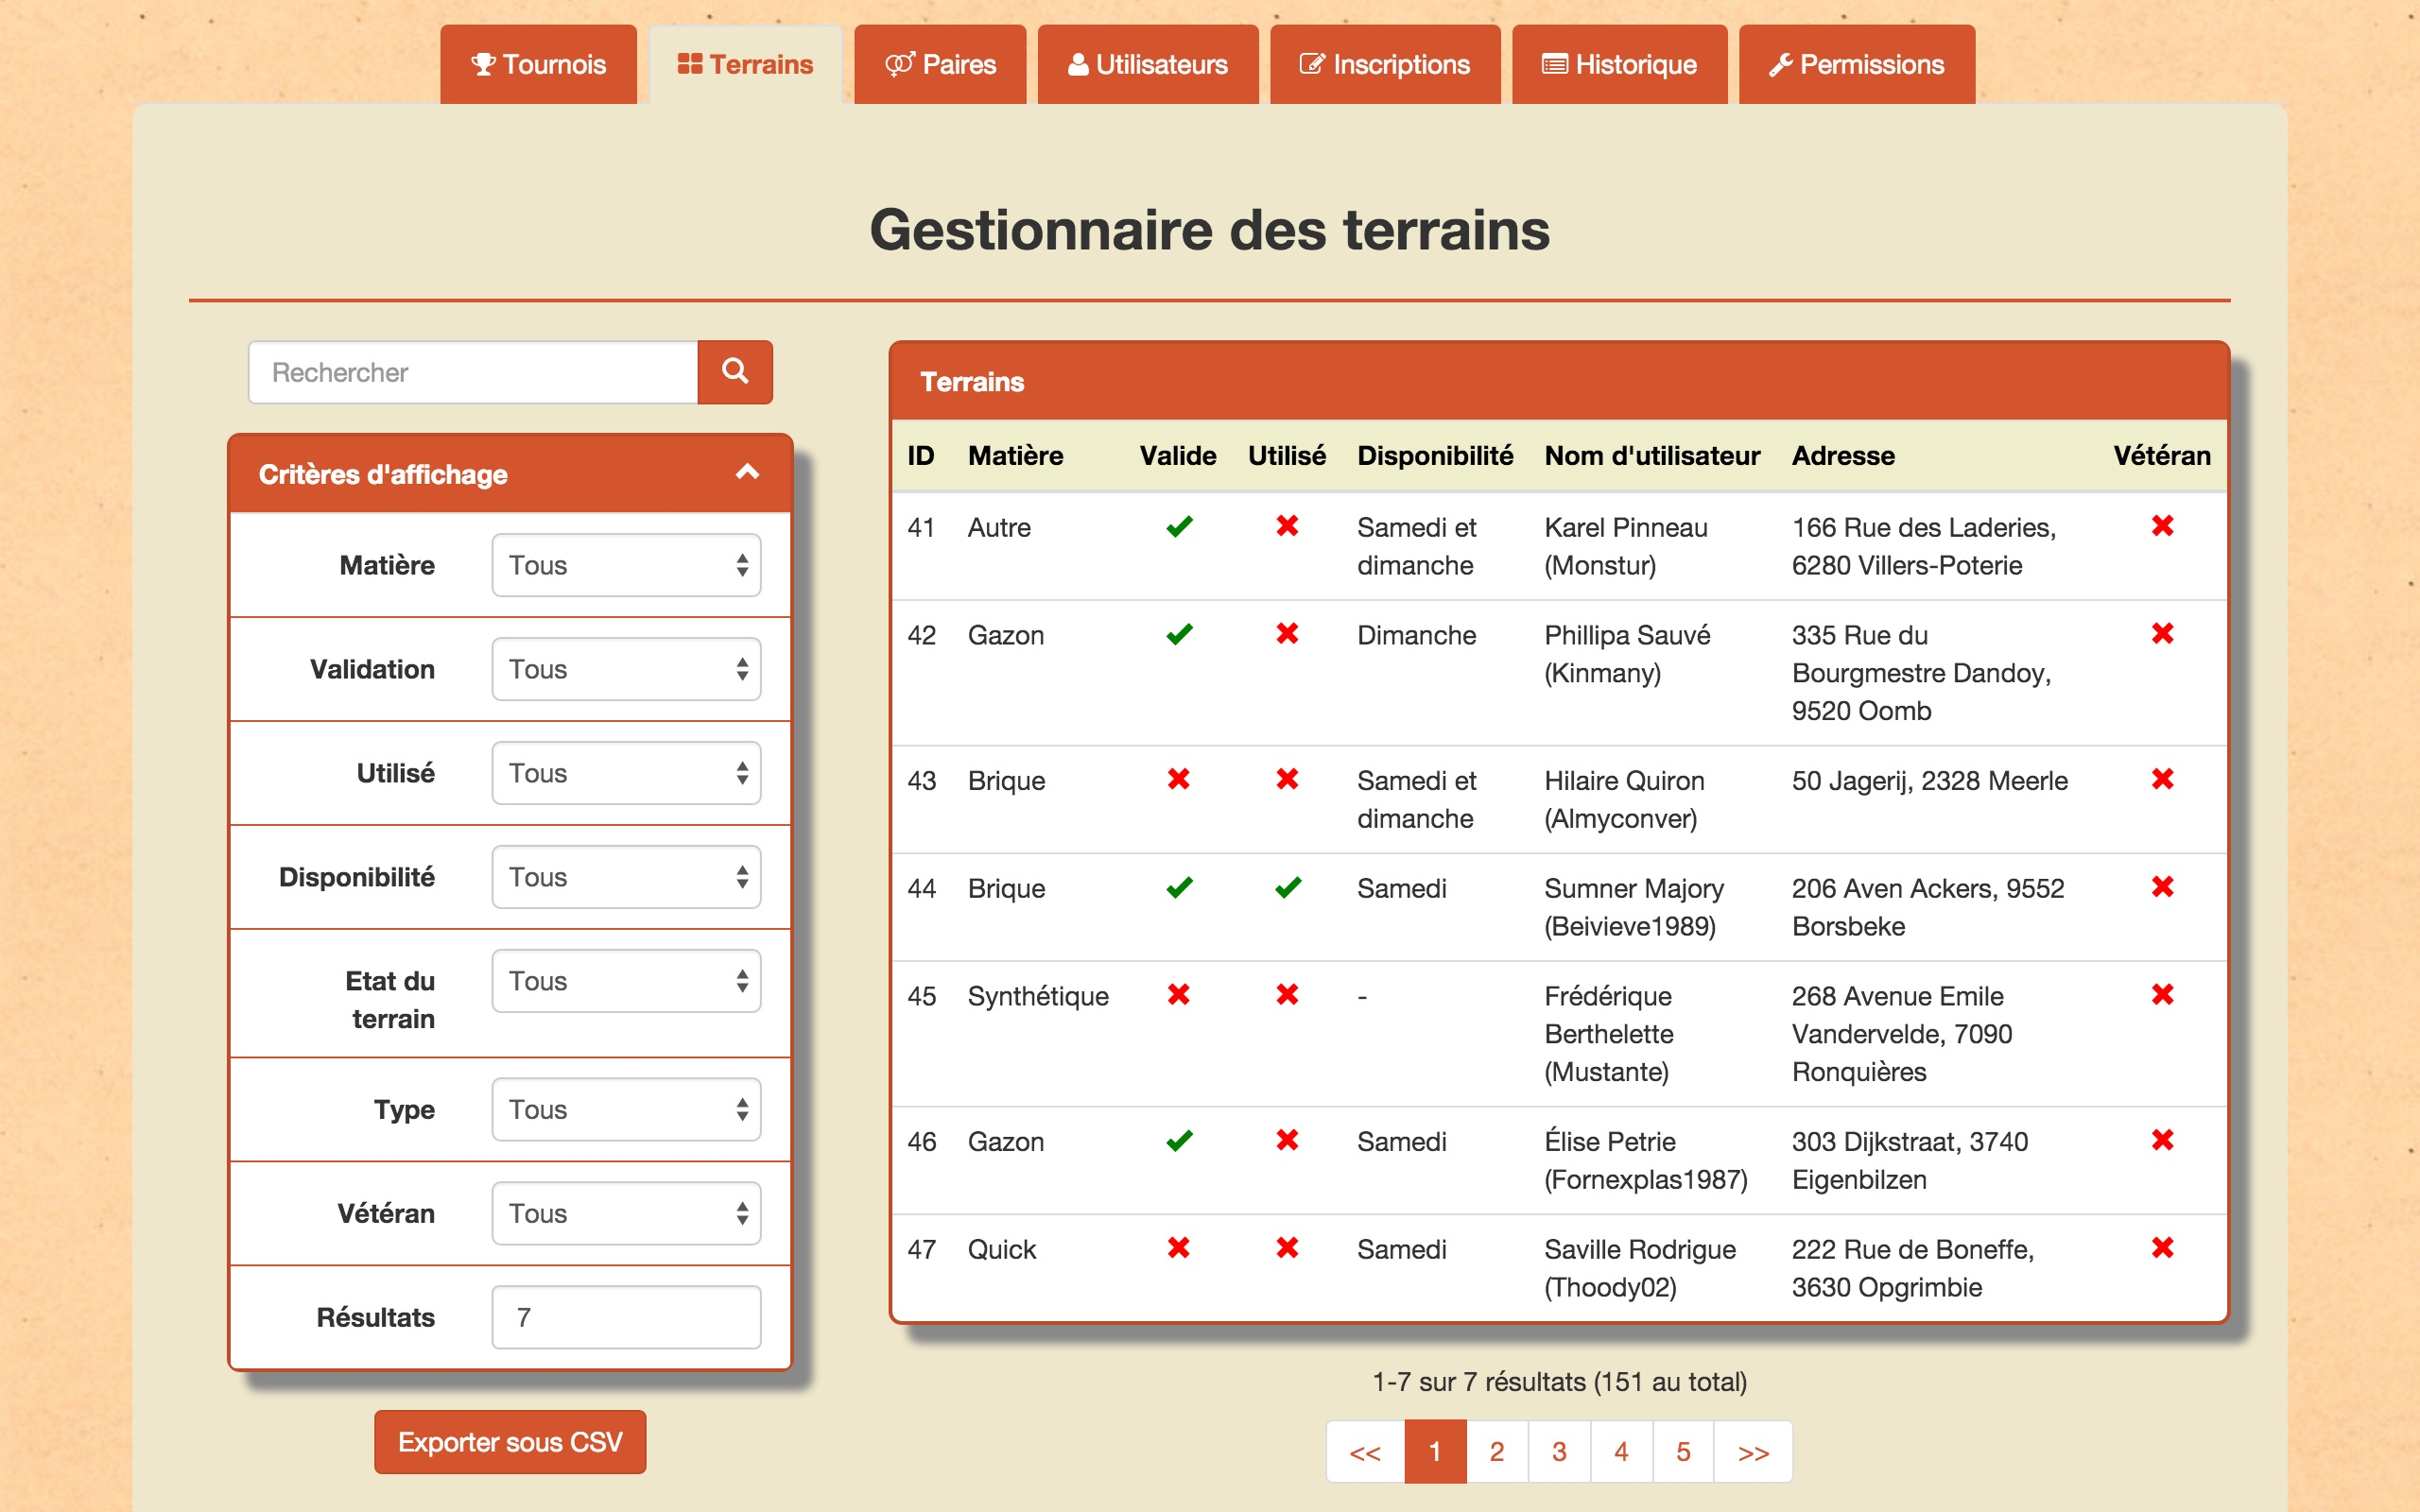
\includegraphics[scale=0.15]{gestion-terrains/gestion-terrains.jpg}
\caption{Page staff principale pour la gestion des terrains}
\end{figure}

\subsection{Les terrains}

Depuis la page staff \enquote{Gestionnaire des terrains}, vous pouvez gérer tous les terrains qui se trouvent dans la base de données. Pour donner la permission à un utilisateur de gérer les terrains, l'admin doit lui octroyer les permissions à partir de la page \enquote{Gestionnaire des permissions} \ref{Gestion des permissions}.\newline

Sur cette page, vous pouvez rechercher des terrains, consulter un terrain, l'éditer, le valider, et le supprimer.\newline

La page principale de la gestion des terrains est divisée en 2 parties :

\begin{itemize}
\item \textit{à gauche}, un champ et des critères de recherche, et un bouton pour exporter la liste des terrains au format CSV ;
\item \textit{à droite}, la liste des terrains qui respectent les critères choisies, et possédant certaines données qui ont une correspondance partielle avec le texte entré dans le champ de recherche
\end{itemize}
\bigskip

Les critères d'affichage des terrains sont les suivants :

\begin{itemize}
\item \textbf{Matière} permet de choisir la matière du terrain ;
\item \textbf{Validation} permet de filter les terrains qui sont validés ou non par le staff ;
\item \textbf{Utilisé} permet de filter les terrains qui sont utilisé dans un tournoi ;
\item \textbf{Disponibilité} permet de filter les terrains par jours disponibles ;
\item \textbf{État du terrain} permet de filter les terrains selon leur état ;
\item \textbf{Type } permet de filter les terrains selon qu'ils sont couverts ou non ;
\item \textbf{Vétéran} permet de filter les terrains selon qu'ils aient déjà été enregistré les années précédentes ou non ;
\item \textbf{Résultats} permet d'indiquer le nombre de terrains à afficher à la fois par page dans la liste des terrains à droite ;
\end{itemize}
\bigskip

Pour effectuer une recherche, il faut sélectionner les critères et entrer le champ de recherche souhaité, puis valider la recherche en cliquant soit sur le bouton de la loupe, soit en appuyant sur la touche \textit{Entrée} du clavier. Le module des critères de recherche peut être minimisé, à tout moment, en cliquant sur le bouton dans le coin droit supérieur du module en forme de \enquote{V} (inversé si la liste des critères sont visibles).\newline

Pour consulter un terrain, il suffit de cliquer sur l'entrée de la liste des terrains contenant les informations du terrain que l'on souhaite consulter. Par exemple, pour consulter le terrain avec l'ID 41, il suffit de cliquer sur la ligne de la liste des terrains où la valeur 41 se trouve dans la colonne ID.

\subsection{Gestion d'un terrain}

\begin{figure}[H]
\centering
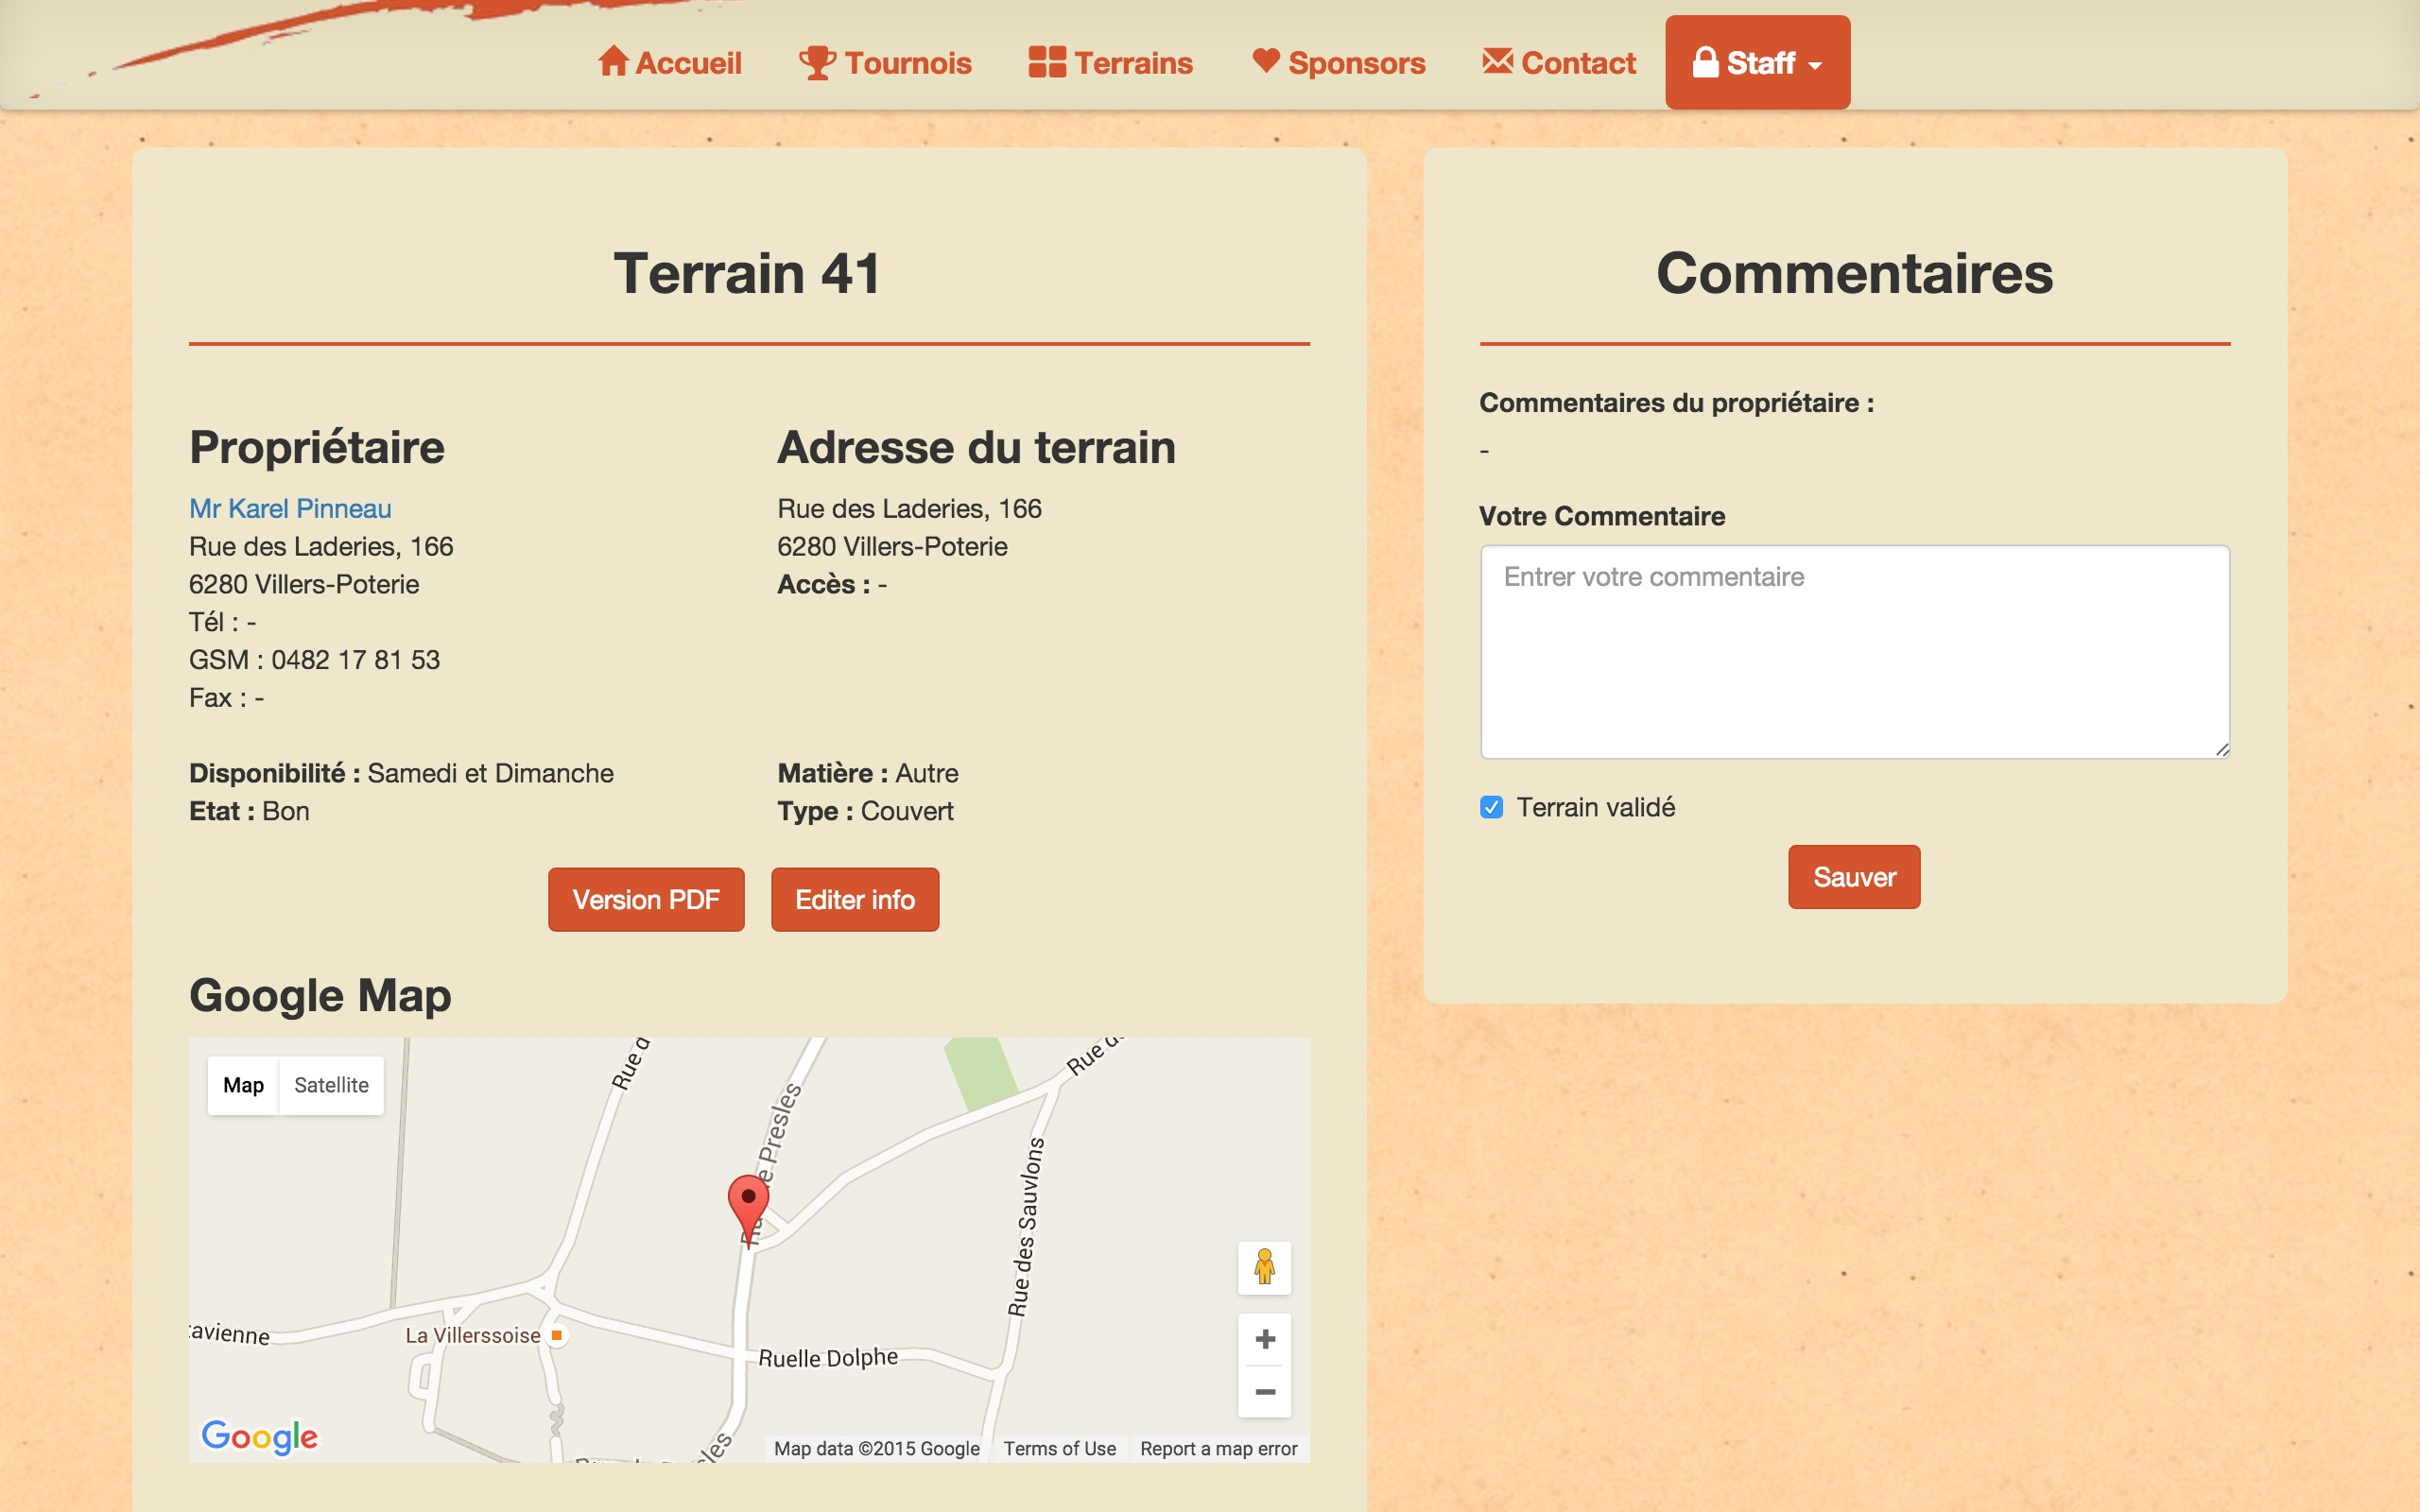
\includegraphics[scale=0.15]{gestion-terrain/gestion-terrain.jpg}
\caption{Page staff de la gestion d'un terrain}
\end{figure}

La page de la gestion d'un terrain se présente en deux modules :

\begin{itemize}
\item \textit{le module de gauche}, qui contient toutes les coordonnées du terrain, ainsi que des boutons d'interaction \textit{Version PDF} (pour télécharger les informations du terrain au format PDF), et \textit{Editer Info} (pour éditer le terrain) ;
\item \textit{le module de droite}, qui contient les commentaires du propriétaire, du staff (éditable), une case cochable pour indiquer si le terrain est valide ou non pour être utilisé dans les tournois, et un bouton \textit{Sauver} pour enregistrer les modifications effectuées dans ce module
\end{itemize}
\bigskip

\textbf{Pour valider ou commenter un terrain}, il suffit de remplir le petit formulaire du module de droite, puis de cliquer sur le bouton \textit{Sauver} pour appliquer les modifications sur les commentaires et/ou sur l'état de validation du terrain. Un terrain validé permet de rendre ce terrain utilisable dans la liste des terrains disponibles pour les tournois, au moment de gérer les poules ou les arbres d'élimination.\newline

\textbf{Pour éditer un terrain}, il suffit de cliquer sur le bouton \textit{Editer info} du module de gauche pour accéder à un formulaire d'édition des informations du terrain, pré-rempli avec les informations actuelles du terrain. Pour appliquer les modifications des informations sur le terrain, cliquez sur le bouton \textit{Editer} en bas de page. Le bouton \textit{Supprimer}, quant à lui, permet de supprimer définitivement le terrain de la base de données. Cette action est irréversible, d'où une boîte de dialogue qui demande à l'utilisateur de confirmer son choix de supprimer le terrain.

\begin{figure}[H]
\centering
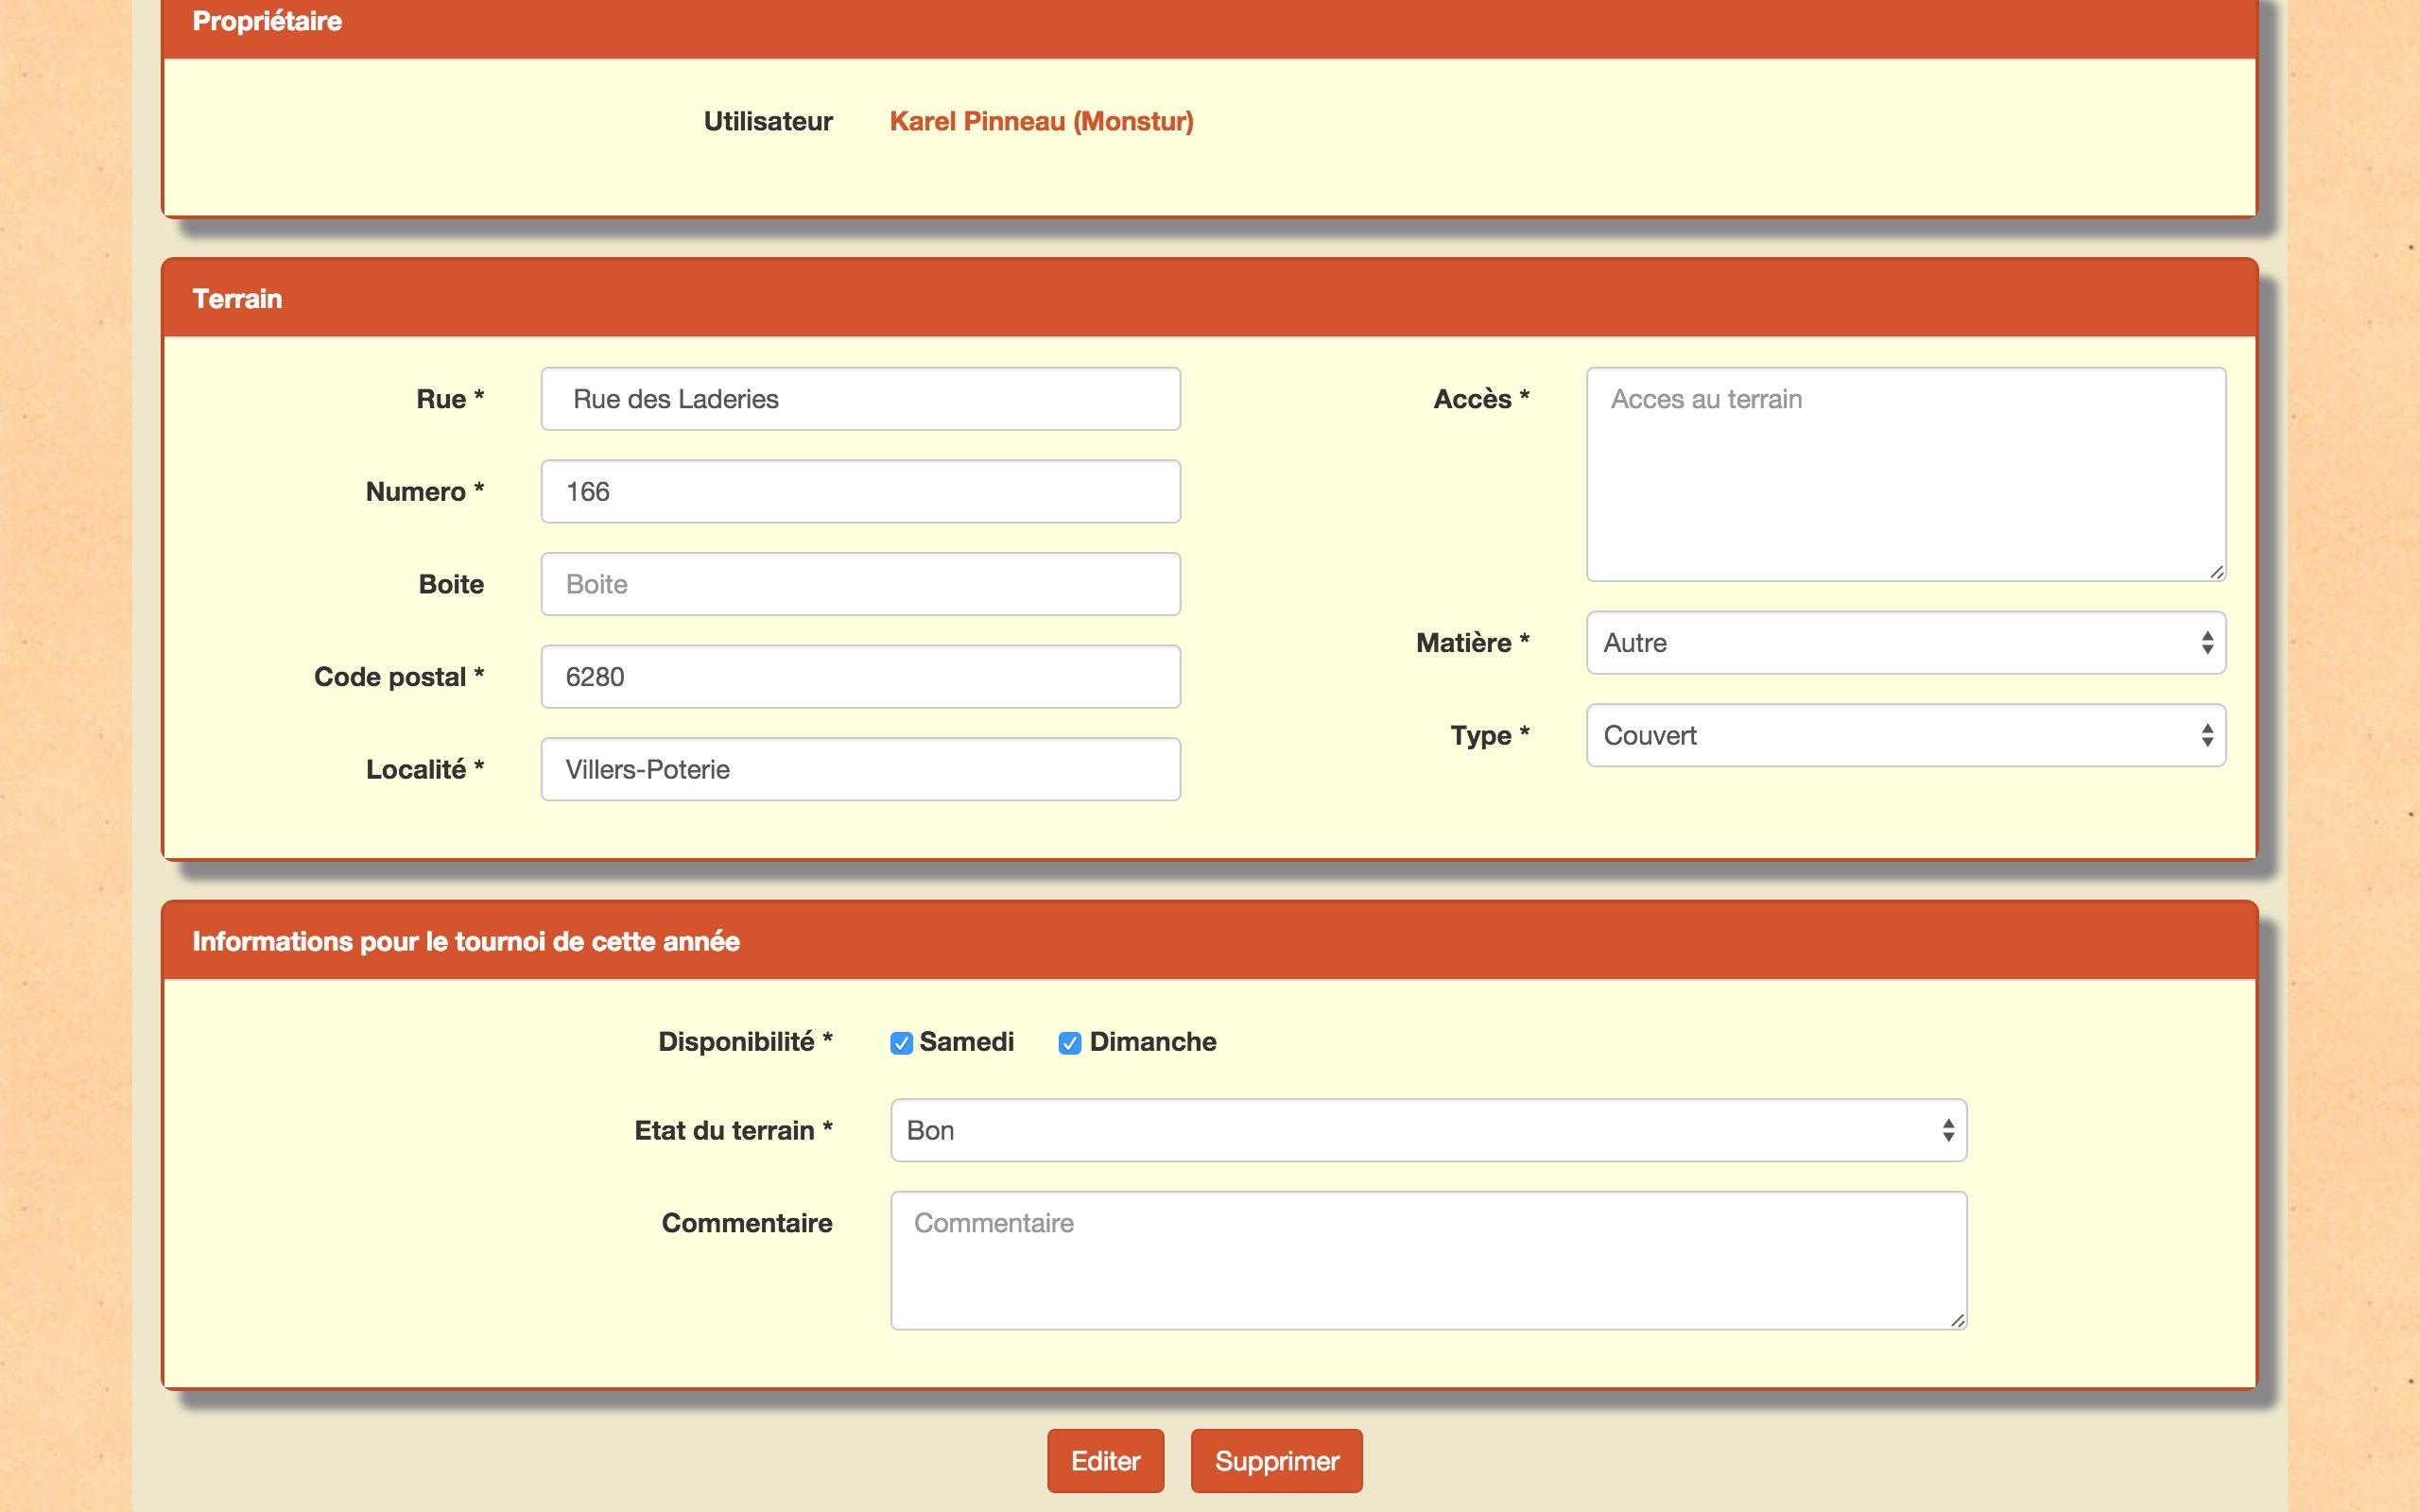
\includegraphics[scale=0.15]{gestion-terrain/gestion-terrain-edition.jpg}
\caption{Page staff de l'édition d'un terrain}
\end{figure}
